% 1988 年全国卷理科第 22 题：正三棱锥及中点
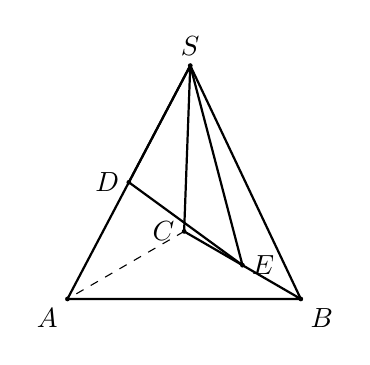
\begin{tikzpicture}[scale=0.78,>=stealth]
  \coordinate (S) at (2.0,3.8);
  \coordinate (A) at (0,0);
  \coordinate (B) at (3.8,0);
  \coordinate (C) at (1.9,1.1);
  \coordinate (D) at (1.0,1.9);
  \coordinate (E) at (2.85,0.55);
  \draw[thick] (S)--(A) (S)--(B) (S)--(C);
  \draw[thick] (A)--(B) (B)--(C);
  \draw[dashed] (C)--(A);
  \draw[thick] (S)--(E) (D)--(E) (S)--(D);
  \fill (S) circle (1.1pt) node[above] {$S$};
  \fill (A) circle (1.1pt) node[below left] {$A$};
  \fill (B) circle (1.1pt) node[below right] {$B$};
  \fill (C) circle (1.1pt) node[left] {$C$};
  \fill (D) circle (1.1pt) node[left] {$D$};
  \fill (E) circle (1.1pt) node[right] {$E$};
\end{tikzpicture}
